\begin{figure}[H]
  \centering

  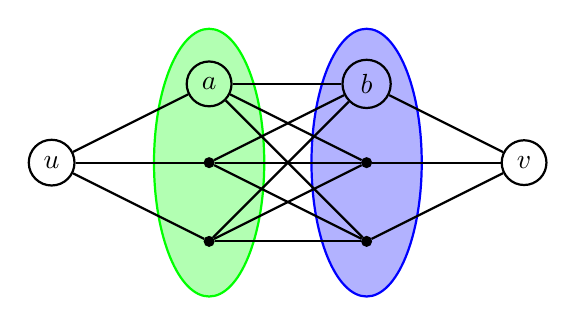
\begin{tikzpicture}[
    dot/.style = {
      shape = circle,
      fill = black,
      minimum size = 4pt,
      inner sep = 0pt,
      outer sep = 0pt,
    },
    point/.style = {
      circle,
      draw = black
    },
    every path/.style = {
      thick
    }
  ] 
    \draw[draw = green, fill = green!30] (2, 0) ellipse (0.7cm and 1.7cm);
    \draw[draw = blue, fill = blue!30] (4, 0) ellipse (0.7cm and 1.7cm);
  
    \node[point] (u) at (0, 0) {\(u\)};
    \node[point] (v) at (6, 0) {\(v\)};
  
    \node[point] (l1) at (2, 1) {\(a\)};
    \node[dot] (l2) at (2, 0) {};
    \node[dot] (l3) at (2, -1) {};
  
    \node[point] (r1) at (4, 1) {\(b\)};
    \node[dot] (r2) at (4, 0) {};
    \node[dot] (r3) at (4, -1) {};
    
    \foreach \idx in {1, 2, 3} {
      \draw (u) -- (l\idx);
      \draw (l\idx) edge (r1) edge (r2) edge (r3);
      \draw (r\idx) -- (v);
    }
  \end{tikzpicture}  
\end{figure}